\chapter[Structural Properties and Clustering]{Structural Properties\\and Clustering}

\section{Features and Network Perturbation}
\label{sec:features_perturbation}

The structural and functional characteristics of complex networks, along with their constituent elements such as nodes, links, communities, and paths, exhibit properties that are deeply intertwined with the nature of the studied system. These properties dictate the fundamental topological structure and the underlying construction rules of the network. In network science, these characteristics can be assessed through two primary approaches. Firstly, they can be directly measured using standard topological metrics, such as various forms of node centrality. Alternatively, they can be deduced dynamically by perturbing the network and rigorously studying the resultant effects on its structure and functionality. The types of perturbations applied can vary significantly; while some perturbation methods are considered "universal" and applicable across diverse topologies, others are strictly model-specific and tailored to particular complex systems.

\subsection{Perturbation of Connectivity}
\label{subsec:perturbation_connectivity}

A fundamental method to understand network resilience and component importance is to test the system's response to connectivity perturbations. These perturbations are generally categorized into two distinct paradigms: random perturbations, commonly referred to as \textit{errors} or failures, and intentional perturbations, known as \textit{attacks}.

The behavioral response of a network to such disruptive events is strongly influenced by the relationships between connected nodes, particularly governed by network assortativity and mixing patterns. By systematically applying these perturbations, researchers can extract valuable information utilized for node relevance classification and for identifying the inherent clustering or community structure within the network.

\subsection{Error and Attack Tolerance}
\label{subsec:error_attack_tolerance}

When nodes are randomly removed from a network, the system's ability to maintain its global connectivity—its tolerance—becomes a subject of critical interest. The network's topology plays a fundamental role in determining this tolerance. Key topological determinants include the degree distribution, which dictates the presence of hubs, and the existence of cycles and multiple paths, which provide necessary structural redundancy.

\begin{figure}[H]
    \begin{minipage}{0.6\textwidth}
        \centering
        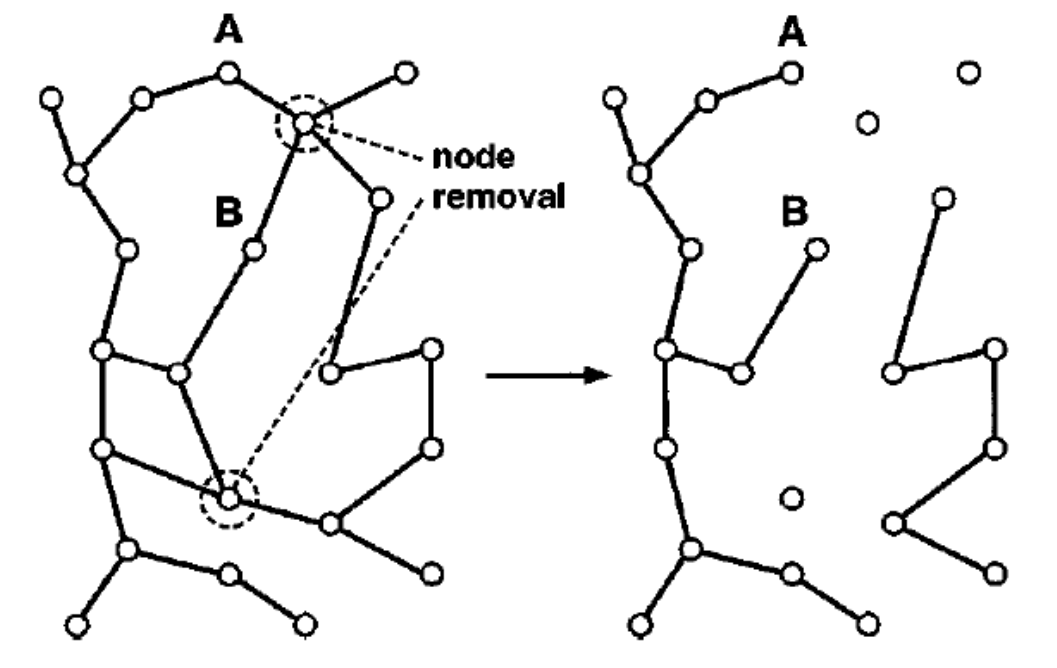
\includegraphics[width=0.8\textwidth]{img/8-tolerance.png}
    \end{minipage}
    \hfill
    \begin{minipage}{0.35\textwidth}
        \caption{Schematic representation of network tolerance under node removal. The left panel illustrates a network with a well-connected structure, while the right panel shows the same network after the removal of a critical node (highlighted in red), resulting in fragmentation and loss of connectivity.}
    \end{minipage}
\end{figure}

\subsubsection{The Percolation Analogy}
The phenomenon of network tolerance under node removal shares a profound theoretical analogy with the percolation process in statistical physics. In this context, nodes (and their incident links) are continuously removed up to a certain \textit{critical density}. Beyond this critical threshold, the macroscopic connectivity collapses, and the network abruptly splits into isolated, separate clusters. In large networks (where the number of nodes $N \gg 1$), this breakdown manifests as a distinct phase transition.

To formalize the terminology:
\begin{itemize}
    \item \textbf{Error}: Denotes the random removal of nodes or links, simulating natural failures.
    \item \textbf{Attack}: Denotes the targeted removal of specific components, usually those of high topological importance.
\end{itemize}

\subsubsection{Tolerance in Erdős-Rényi (E-R) and Barabási-Albert (B-A) Networks}

The response to errors and attacks varies dramatically depending on the network generation model.

For homogeneous networks, such as the Erdős-Rényi (E-R) random graph model, error tolerance is mathematically linked to the percolation threshold. The fragmentation represents a phase transition similar to standard percolation, and the process is fundamentally reversible (representing the inverse of the Giant Component transition). In E-R networks, because all nodes are statistically equivalent, targeted attacks based on node degree produce damage at a slightly faster rate, but the overall network breakdown behavior does not differ drastically from that observed under random random removal. Ultimately, a homogeneous E-R network is highly susceptible to breaking down into separate clusters under random errors.

Conversely, scale-free networks generated by the Barabási-Albert (B-A) model exhibit vastly different dynamics due to their extreme node heterogeneity. For random node removal, the critical threshold for B-A networks asymptotically tends to 1 in the thermodynamic (TD) limit; effectively, almost all nodes must be removed to completely disconnect the network, meaning there is no standard phase transition. This makes scale-free networks exceptionally robust to random errors, primarily because the probability of randomly selecting and removing a critical hub is statistically very low.

However, this robustness comes at a severe cost regarding attack tolerance. When an \textit{attack} strategy is employed—specifically removing nodes sorted by descending degree—the B-A network proves to be exceedingly fragile. Removing the hubs drastically and rapidly destroys the global connectivity, resulting in a much lower breakdown threshold compared to random failures. In scale-free topologies, hubs are the critical lynchpins of the system.

\begin{figure}[H]
    \centering
    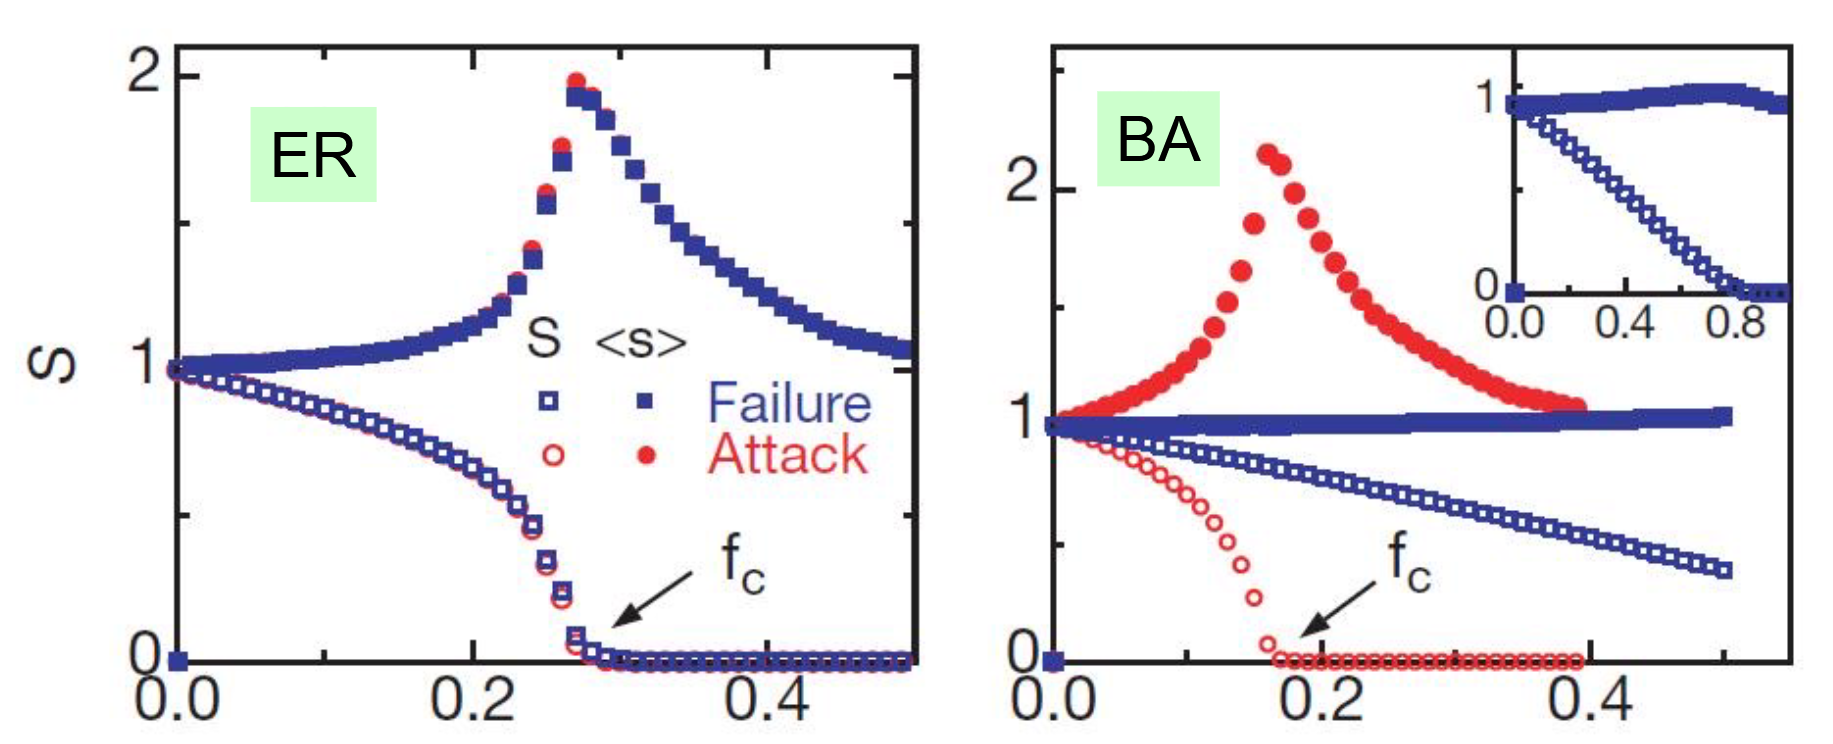
\includegraphics[width=0.8\textwidth]{img/8-tolerance_comparison.png}
    \caption{Comparative analysis of network tolerance (fragmentation parameter $S$ and average cluster size \(\langle s \rangle\) ) under random failures and targeted attacks for Erdős-Rényi (E-R) and Barabási-Albert (B-A) networks. The left panel illustrates the gradual fragmentation of an E-R network under random node removal (as a function of the fraction of removed nodes $f_c$), while the right panel demonstrates the rapid collapse of a B-A network when hubs are targeted for removal.}
\end{figure}

\subsection{Real Networks: Empirical Analysis}
\label{subsec:empirical_analysis}

In practical applications and real-world empirical analyses, network perturbation serves as a powerful diagnostic tool to quantify node relevance. By systematically removing nodes, one can observe and measure the magnitude of change across various network dimensions:
\begin{itemize}
    \item \textbf{Global properties}: Observing changes in the size of the largest connected component or the overall global efficiency of the network.
    \item \textbf{Spectral properties}: Tracking variations in eigenvalues, such as the Fiedler Number (algebraic connectivity).
    \item \textbf{Community structure}: Analyzing how perturbations alter the size, number, and boundaries of network communities.
\end{itemize}

Beyond simple degree-based attacks, empirical analyses often consider more sophisticated strategies for node removal to uncover deeper structural vulnerabilities. These advanced strategies include removing nodes sorted by other centrality measures (such as betweenness or eigenvector centrality), or executing simultaneous multi-node removals. Simultaneous removals can be strategically targeted based on a node's specific position within the community structure (e.g., removing boundary spanners) or based on topological proximity, such as removing a targeted node along with its immediate neighborhood.

\section{Node Correlation and Assortativity}
\label{sec:node_correlation_assortativity}

While global topological metrics such as the degree distribution $P(K)$ provide fundamental insights into the overall structure of a complex network, they are insufficient to fully characterize its wiring diagram. Specifically, knowing the degree of nodes does not explain the underlying relationships between them. Given two networks with an identical degree distribution, the microscopic connectivity can vary drastically based on whether nodes connect to each other purely at random or if there are inherent link preferences.

Therefore, a crucial feature to analyze is node correlation. In many real-world systems, relationships are not established uniformly; instead, there may be heavily favored or distinctly disadvantaged connections between specific pairs or classes of nodes.

\subsection{Node Types and Labeling}
\label{subsec:node_types_labeling}

To formalize the study of link preferences, we often categorize nodes into distinct groups based on specific characteristics, essentially associating different \textit{labels} (usually known a priori) with the various types of nodes within the network. This process is known as node labeling.

The nature of these relationships and the resulting node types vary depending on the system under study. Examples of node relations classified by discrete labels include:
\begin{itemize}
    \item \textbf{Biological networks}: Differentiating proteins that share the same biological functions or belong to specific protein families.
    \item \textbf{Social networks}: Categorizing individuals by sex, social classes, distinct social groups, or spoken language.
    \item \textbf{Technological and Information networks}: Grouping websites by topic or classifying nodes based on specific physical-chemical parameters.
    \item \textbf{Spatial networks}: Defining nodes by their spatial position, such as streets, cities, or tracking the spatial distribution of migrating animals.
\end{itemize}

\subsection{Mixing and Correlation}
\label{subsec:mixing_correlation}

Once labels are assigned, we can quantitatively characterize the amount of connectivity—or \textit{mixing}—between nodes that share the same label versus those with different labels. This provides a clear mathematical picture of network stratification, illustrating how connectivity behaves as a function of specific node characteristics.

\subsubsection{The Mixing Matrix}

The most direct way to represent these correlations is by counting the number of connections between intra-group nodes and inter-group nodes.

Consider a simplified example of a network containing nodes with two distinct labels, "A" and "B". We can construct a mixing matrix $M_{AB}$ where the elements represent the total number of links connecting specific groups:
$$M_{AB} = N_{K(AB)} \qquad \begin{pmatrix} M_{AA} & M_{AB} \\ M_{BA} & M_{BB} \end{pmatrix}$$

More generally, if a network features $N$ distinct labels, the mixing behavior is captured by an $N \times N$ matrix.

To determine whether the observed mixing is significant, we must compare it against a \textit{null model}. In a completely random mixing scenario, the number of connections is purely a function of the total number of nodes and available links for each labeled group. In our two-label example, if links were distributed randomly without preference, the expected number of links between groups would be strictly proportional to the product of their sizes: $N_A \times N_A$ for group A, $N_B \times N_B$ for group B, and $N_A \times N_B$ for cross-connections. Deviations from this proportional expectation indicate the presence of significant network correlation.

\subsubsection{The E-Matrix and Assortativity}

In practice, it is often more useful to work with normalized values rather than absolute counts. We define the matrix $E$ (often denoted by its elements $e_{ij}$) representing percentages over the total number of links in the network:
\begin{itemize}
    \item $e_{ii}$ represents the fraction of links connecting nodes \textit{within} the same community $i$.
    \item $e_{ij}$ represents the fraction of links connecting a node in community $i$ to a node in community $j$.
\end{itemize}

By definition, the sum of all elements in the E-matrix must equal 1:
$$\sum_{ij} e_{ij} = 1$$

Furthermore, we can define the marginal sums, $a_i$ and $b_j$, which represent the percentage of links connecting community $i$ (or $j$) to all other communities:
$$\sum_{j} e_{ij} = a_i$$
$$\sum_{i} e_{ij} = b_j$$

Using these normalized fractions, we can quantify the overall level of assortative mixing in the network using the assortativity coefficient, $r$. This coefficient compares the observed trace of the E-matrix (the fraction of intra-group links) against the expected value under the random mixing null model ($\sum_{i} a_i b_i$):

$$r = \frac{\sum_{i} e_{ii} - \sum_{i} a_i b_i}{1 - \sum_{i} a_i b_i} = \frac{\mathrm{Tr}(e) - \|e^2\|}{1 - \|e^2\|}$$

The value of the assortativity coefficient is bounded such that $-1 \le r \le 1$.
\begin{itemize}
    \item If $r = 1$, the network is perfectly assortative: all links exist exclusively within the same groups ($e_{ii}$ is maximized).
    \item If $r = -1$, the network is perfectly disassortative: there are absolutely no links within the same group (all connections are inter-group, and the sum $\sum_i a_i b_i = 1/2$).
\end{itemize}

\subsection{Impact on Dynamic Processes: Epidemic Spreading}
\label{subsec:epidemic_spreading}

Network stratification and node correlation severely impact dynamic processes unfolding on the network topology. Understanding mixing patterns is crucial for analyzing the propagation of information, the flow of goods, or the spread of diseases, as correlations create preferred transmission routes while leaving other regions less easily reached.

A prime example is epidemic spreading. In a population, different "node types" exhibit vastly different probabilities of getting into contact. For instance:
\begin{itemize}
    \item \textbf{High-density interactions}: Young people in school environments.
    \item \textbf{Inter-generational mixing}: Contacts between children and parents.
    \item \textbf{Superspreading events}: High-contact environments like shops, workplaces, and bars where a single node can easily transmit to many others across different social groups.
\end{itemize}

Consequently, mixing data is fundamental for designing network immunization strategies. Epidemic spread prevention measures can be vastly improved if they are targeted not just randomly, but by focusing on specific subsets of relations characterized by a higher risk of contagion or targeting specific groups vulnerable to dangerous contagion (e.g., elderly populations). By acting on specific nodes by group based on their mixing patterns, interventions become significantly more effective.

\subsection{Topological Assortativity: Degree Correlation}
\label{subsec:topological_assortativity}

Beyond using external or categorical attributes as node labels (such as biological function or social class), we can utilize intrinsic \textit{topological parameters} of the network itself as labels to evaluate mixing patterns. When doing so, it is important to bear in mind that some topological metrics may be strictly correlated or anti-correlated with each other, rendering them mathematically equivalent in this context.

The most classic and widely studied case of topological labeling is using the node degree, $k$. In this scenario, we investigate whether nodes of a certain degree exhibit a preference to connect with nodes of a similar or dissimilar degree. This requires analyzing the preferential degree of the first neighbor nodes, mathematically expressed as the conditional probability $P(k'|k)$ or simply $p(k, k_{NN})$.

Empirically, this topological assortativity is evaluated by plotting the node degree $k$ against the average degree of its nearest neighbors, denoted as $k_{nn}(k)$ or $\langle K_{NN} \rangle$. The shape of the resulting curve reveals the network's degree correlation profile:
\begin{itemize}
    \item \textbf{Assortativity (Growing Curve)}: A positive correlation indicates that high-degree nodes (hubs) preferentially connect to other hubs, while low-degree nodes connect to other low-degree nodes.
    \item \textbf{Disassortativity (Decreasing Curve)}: A negative correlation signifies that high-degree nodes predominantly connect to low-degree nodes, creating a hub-and-spoke-like architecture.
    \item \textbf{Neutral Assortativity (Flat Curve)}: A lack of correlation indicates that nodes connect regardless of their respective degrees, typical of purely random networks.
\end{itemize}

\begin{figure}[H]
    \centering
    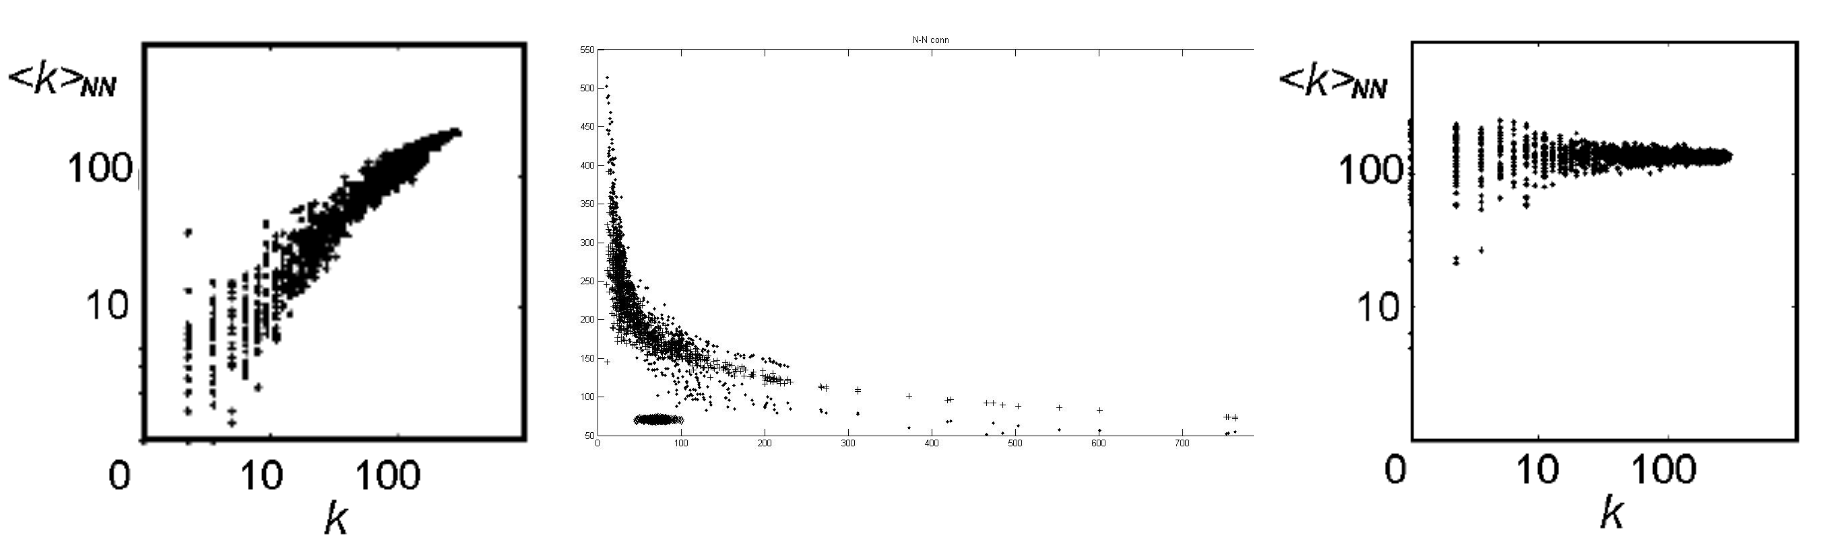
\includegraphics[width=0.8\textwidth]{img/8-assortativity.png}
    \caption{Illustration of degree assortativity patterns in complex networks. The plot shows the average nearest neighbor degree $\langle K_{NN} \rangle$ as a function of node degree $k$ for three different networks: an assortative network (blue curve) exhibiting a positive correlation, a disassortative network (red curve) showing a negative correlation, and a neutral network (green curve) with no correlation.}
\end{figure}

\subsection{Classes of Networks based on Assortativity}
\label{subsec:classes_of_networks}

Extensive empirical analyses of diverse real-world systems have revealed consistent patterns, allowing us to classify networks broadly based on their assortative tendencies.

\subsubsection{Assortative Networks}
Social networks typically exhibit strong assortative mixing. This phenomenon is often driven by mechanisms such as homophily (the tendency of individuals to associate with similar peers) and "triadic closure" (the high probability that two friends of a common friend will also become friends). Because hubs represent highly social individuals, they tend to cluster together, forming dense, highly interconnected cores.

Notable empirical examples include:

\begin{figure}[H]
    \begin{minipage}{0.55\textwidth}
        \begin{itemize}
            \item \textbf{PGP (Pretty Good Privacy)}: A web of trust graph representing secure communications.
            \item \textbf{SCN (Scientific Collaboration Networks)}: Co-authorship networks where prolific authors frequently collaborate with other established researchers.
            \item \textbf{WAN (World Airport Network)}: Often exhibits assortative features due to major hubs (capital cities) heavily routing traffic to other major hubs.
        \end{itemize}
        \caption{Plot showing the growing trend in K vs $\langle K_{PV} \rangle$ (nearest neighbor degree) and the corresponding clustering coefficient K vs C for three different real world assortative networks: PGP, SCN, and WAN.}
    \end{minipage}
    \hfill
    \begin{minipage}{0.4\textwidth}
        \centering
        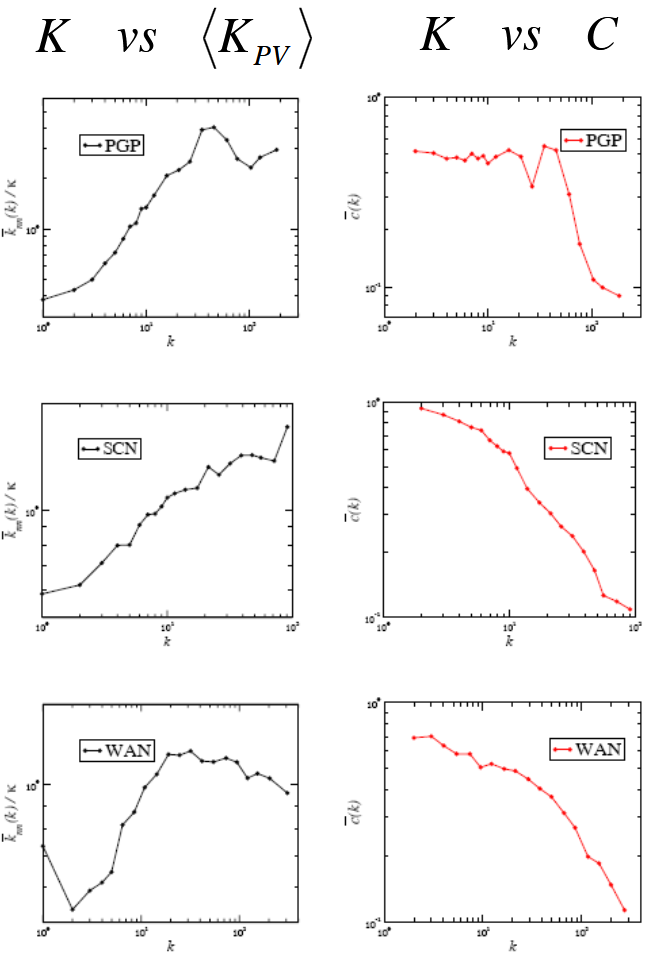
\includegraphics[width=0.9\textwidth]{img/8-assortative_realworld.png}
    \end{minipage}
\end{figure}

\subsubsection{Disassortative Networks}
Conversely, technological and biological networks overwhelmingly tend to be disassortative. These systems are often "regulatory" or hierarchical in nature, optimized for functional distribution rather than social cohesion. In such networks, hubs act as central distributors or regulators interacting with numerous low-degree peripheral nodes, rather than forming cliques with other hubs.
Standard examples include:


\begin{figure}[H]
    \begin{minipage}{0.55\textwidth}
        \begin{itemize}
            \item \textbf{AS (Autonomous Systems)}: The topological routing structure of the Internet.
            \item \textbf{PIN (Protein Interaction Networks)}: Biological networks where highly connected essential proteins usually regulate or interact with specialized, less-connected proteins.
            \item \textbf{WTW (World Trade Web)}: Economic networks where dominant global economies trade extensively with smaller, developing nations.
        \end{itemize}
        \caption{Plot showing the growing trend in K vs $\langle K_{PV} \rangle$ (nearest neighbor degree) and the corresponding clustering coefficient K vs C for three different real world disassortative networks: AS, PIN, and WTW.}
    \end{minipage}
    \hfill
    \begin{minipage}{0.4\textwidth}
        \centering
        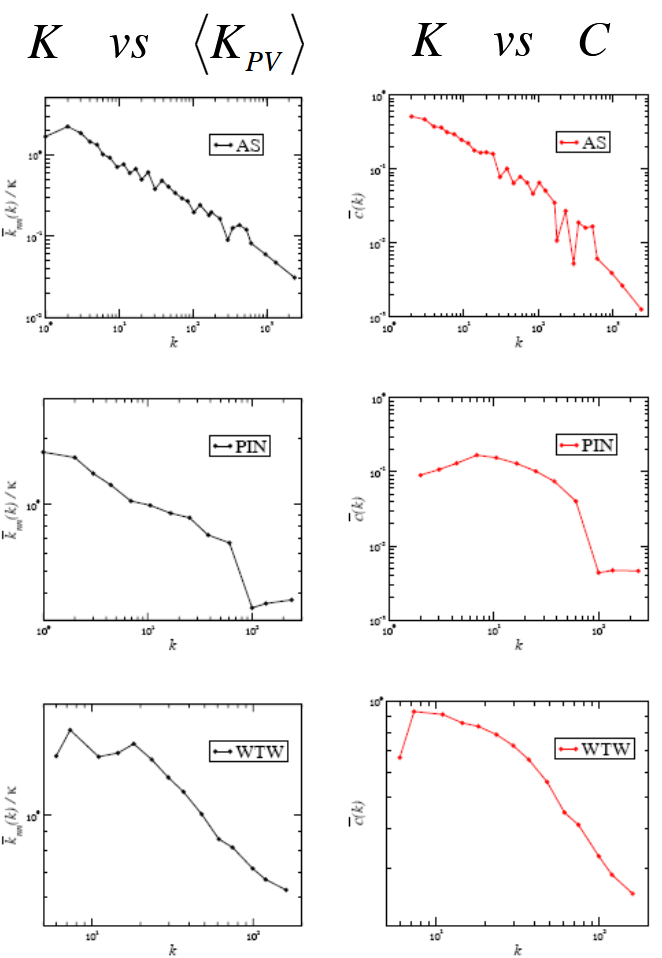
\includegraphics[width=0.9\textwidth]{img/8-disassortative_realworld.png}
    \end{minipage}
\end{figure}

\subsection{Structural Constraints and Null Models}
\label{subsec:constraints_and_null_models}

When evaluating the assortativity of a real network, one must ask whether the observed correlations are due to specific interaction mechanisms or merely artifacts of physical constraints and network construction rules.

For instance, certain network generation models inherently produce correlated structures by "nature." The Barabási-Albert (B-A) scale-free model, driven by preferential attachment, naturally generates highly disassortative networks because new, low-degree nodes are forced to attach to existing high-degree hubs. In contrast, explicitly correlation-based models are designed to generate assortative topologies.

\subsubsection{Defining the Proper Null Model: Link Reshuffling}

To determine the statistical significance of observed assortativity, we must compare the real network against a suitable \textit{null model}. While an Erdős-Rényi (E-R) random graph serves as a basic uncorrelated baseline (yielding a flat $k_{nn}(k)$ curve), it is often insufficient because it destroys the original degree sequence, which fundamentally alters the network's macroscopic properties.

The critical question is: \textit{How can we preserve the global and local connectivity properties of the original network (specifically the degree distribution) while entirely removing high-order correlations?}

The standard solution is the \textbf{Link Reshuffling algorithm} (frequently attributed to Maslov \& Sneppen). This algorithm computationally generates a \textit{microcanonical ensemble} of randomized networks that share the exact same degree sequence as the original network.

The procedure works by randomly selecting two pairs of connected nodes (e.g., $A \rightarrow B$ and $C \rightarrow D$) and swapping their target partners (creating $A \rightarrow D$ and $C \rightarrow B$), provided no multiple edges or self-loops are created. By repeating this process numerous times, the algorithm successfully:
\begin{itemize}
    \item Preserves the strict local connectivity (both in-degree and out-degree of every individual node remain constant).
    \item Eradicates long-range and nearest-neighbor relationships, effectively neutralizing both degree assortativity and the clustering coefficient.
\end{itemize}
By comparing the real network's assortativity to the ensemble average generated by the Maslov-Sneppen reshuffling, researchers can robustly quantify whether the observed topological correlations are functionally significant or purely structural consequences of the degree sequence.

\begin{figure}[H]
    \centering
    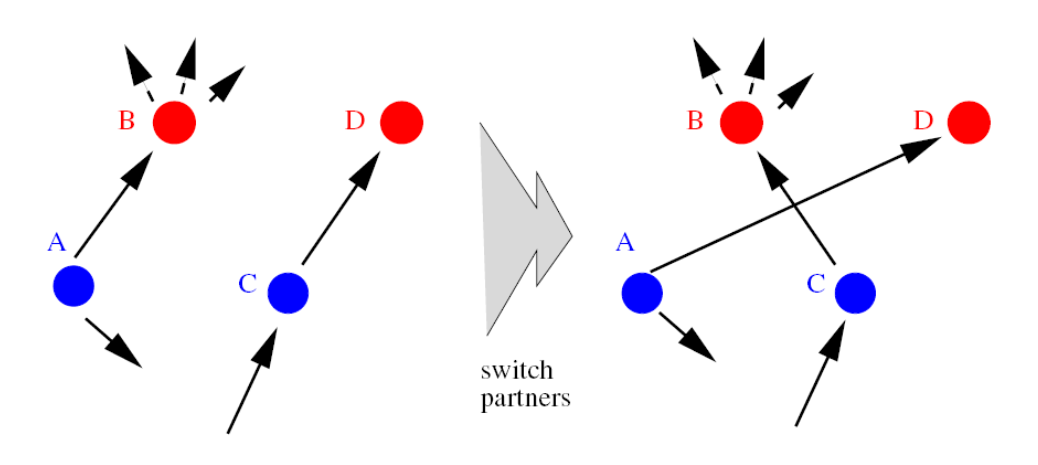
\includegraphics[width=0.8\textwidth]{img/8-link_reshuffling.png}
    \caption{Schematic representation of the Link Reshuffling (Maslov \& Sneppen) process. Two original directed edges (A $\rightarrow$ B and C $\rightarrow$ D) are shown alongside an arrow labeled "switch partners," resulting in two new edges (A $\rightarrow$ D and C $\rightarrow$ B) while preserving the number of stubs for nodes A, B, C, and D.}
\end{figure}

\section{Communities and Clustering}
\label{sec:communities_clustering}

A fundamental characteristic of many real-world complex networks is their modular structure, meaning they inherently organize into communities or clusters. Nodes within these communities feature a high density of internal connections compared to a lower density of external connections between different groups. The methodological approach to finding these structures depends largely on the scale of the topological features being investigated.

When the objective is to find \textit{small communities}, the analysis typically focuses on highly cohesive local structures such as cliques, k-plexes, and recurring network motifs. Conversely, when looking for \textit{large communities} that dictate the macroscopic organization of the system, broader methodologies like graph partitioning and global clustering algorithms are employed.

\subsection{Hierarchical Clustering}
\label{subsec:hierarchical_clustering}

One of the most prevalent paradigms for uncovering large-scale community structure is hierarchical clustering. This method relies on a recursive, agglomerative (bottom-up) partitioning strategy. The output of this process is typically visualized as a dendrogram—a tree-like diagram that records the sequence of merges.

The general algorithm proceeds as follows:
\begin{enumerate}
    \item Define and compute a distance metric $d_{ij}$ between all pairs of nodes in the network, sorting them from shortest to longest.
    \item Iteratively merge the closest nodes (or clusters) into larger clusters.
    \item Continue this progressive merging process until a complete spanning of all available elements is achieved, culminating in a single giant cluster containing all nodes.
\end{enumerate}
Once the dendrogram is constructed, a horizontal "cut" across the branches determines the final cluster boundaries and the total number of distinct communities.

\begin{figure}[H]
    \begin{minipage}{0.6\textwidth}
        \centering
        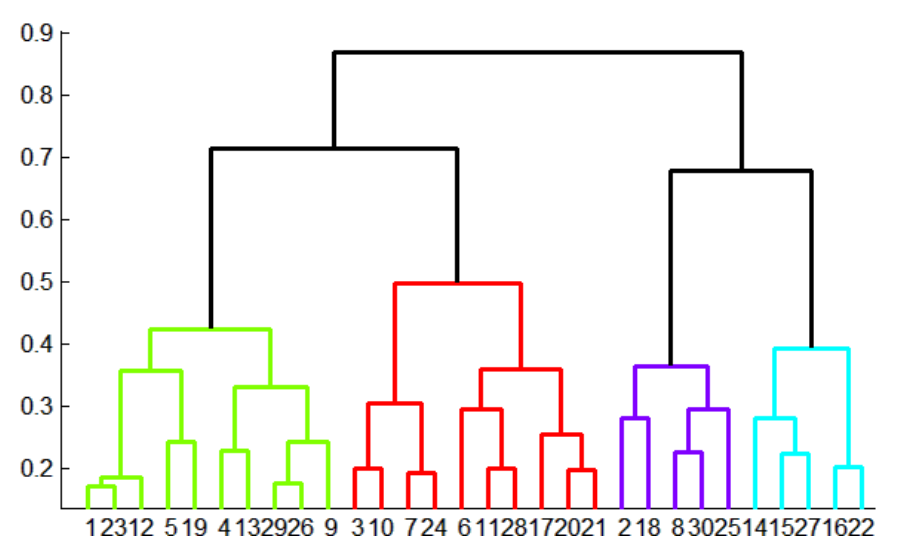
\includegraphics[width=0.9\textwidth]{img/8-dendrogram.png}
    \end{minipage}
    \hfill
    \begin{minipage}{0.35\textwidth}
        \caption{Illustration of a dendrogram resulting from hierarchical clustering. The vertical axis represents the distance at which clusters are merged, while the horizontal axis represents the individual nodes and their subsequent merges into larger clusters. Distinct sub-trees (separate communities) highlighted in different colors (e.g., green, red, purple, cyan).}
    \end{minipage}
\end{figure}

\subsubsection{Defining the Distance Metrics}
\label{subsubsec:distance_metrics}

The foundation of hierarchical clustering is the distance function, which quantitatively defines how "close" or "similar" two nodes are. Several metrics can be employed:

\paragraph{1. Weighted Node Distance:} The most intuitive metric is the shortest path between nodes. In weighted networks, this translates to finding the paths utilizing the strongest links. As nodes are grouped, this concept extends to measuring the shortest distance between entire clusters, where a higher inter-cluster link density effectively increases the weight (reduces the distance) between them.

\paragraph{2. Structural Equivalence:} This metric posits that nodes are structurally equivalent, and thus closer, if they share a similar local neighborhood. Mathematically, it is evaluated by computing the Euclidean distance (or the Pearson correlation) between the corresponding rows or columns of the adjacency matrix $A$.

The Euclidean distance $D_{ij}$ between nodes $i$ and $j$ is given by:
$$D_{ij} = \sqrt{ \sum_{k=1, k\neq i,j}^{N} (a_{ik} - a_{jk})^2 }$$

Alternatively, the Pearson correlation coefficient $R_{ij}$ normalizes this relationship:
$$R_{ij} = \frac{\sum_{k=1}^{N}(a_{ik} - \bar{a}_i)(a_{jk} - \bar{a}_j)}{\sqrt{\sum_{k=1}^{N}(a_{ik} - \bar{a}_i)^2} \sqrt{\sum_{k=1}^{N}(a_{jk} - \bar{a}_j)^2}}$$

\paragraph{3. Topological Overlap of Matrices (TOM):} This advanced metric quantifies similarity based on the number of common neighbors two nodes share. The topological overlap distance $d_N(i,j)$ is defined as:
$$d_N(i,j) = \frac{|N_N(i) \cap N_N(j)| + a_{ij}}{\min(|N_N(i)|, |N_N(j)|) + 1 - a_{ij}}$$

Where the intersection of neighbors is strictly the dot product of their adjacency vectors:
$$|N_N(i) \cap N_N(j)| = \sum_k a_{ik} \cdot a_{jk}$$
Furthermore, the minimum degree constraint is simply $\min(k_i, k_j)$.

\subsubsection{Linkage Criteria}
\label{subsubsec:linkage}

When computing distances between newly formed multi-node clusters, a merging rule—or \textit{linkage criterion}—must be defined to represent the cluster-to-cluster distance.

\begin{itemize}
    \item \textbf{Single Linkage:} Joins clusters based on the \textit{smallest} distance between their closest respective nodes.
    \item \textbf{Complete Linkage:} Joins clusters based on the \textit{smallest} distance between their \textit{furthest} respective nodes.
    \item \textbf{Average Linkage:} Joins clusters based on the average distance across all node pairs between the two clusters.
\end{itemize}

\begin{figure}[H]
    \centering
    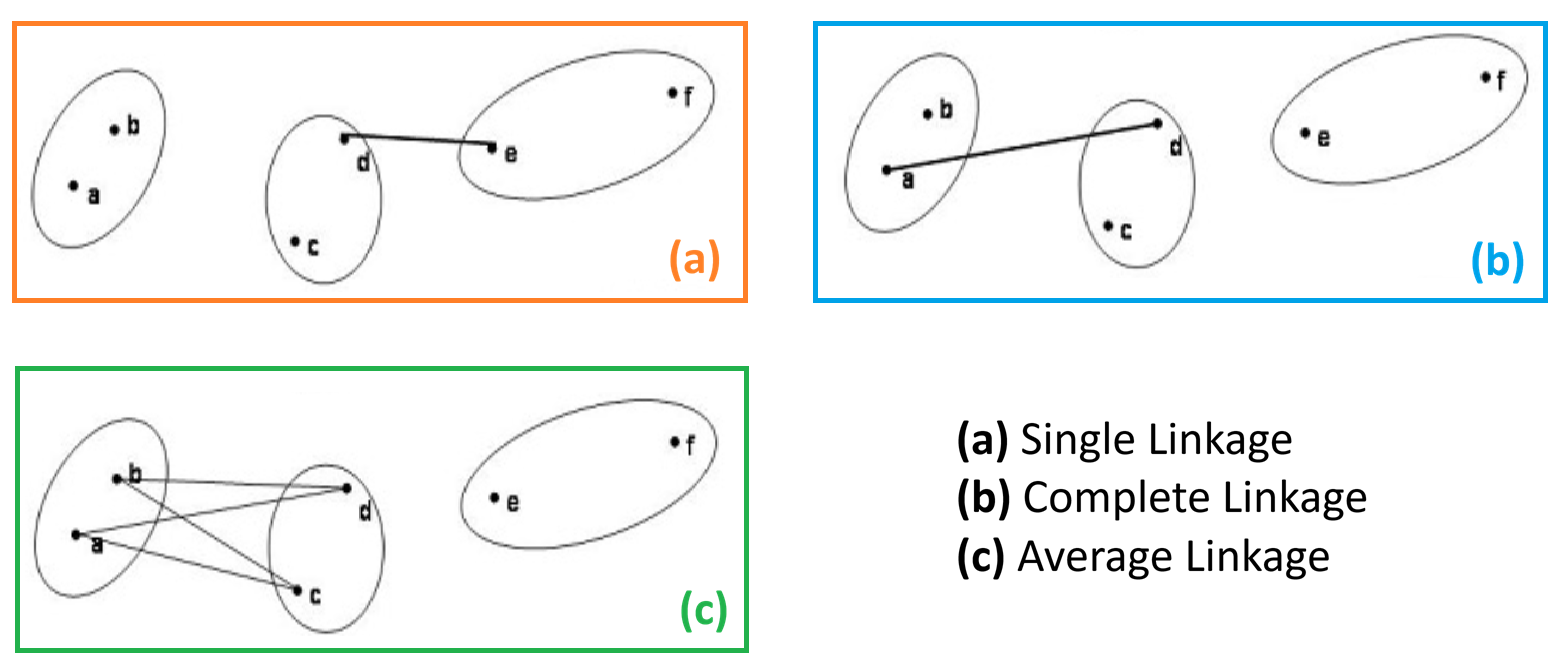
\includegraphics[width=0.8\textwidth]{img/8-linkage.png}
    \caption{Illustration of different linkage criteria in hierarchical clustering. The diagram shows three clusters with various inter-node distances.}
\end{figure}

\begin{figure}[H]
    \begin{minipage}{0.5\textwidth}
        The choice of linkage drastically affects the resulting community structure. Single linkage often suffers from a "chaining" effect, where resulting clusters tend to form long, uninformative chains. Complete linkage performs exceptionally well if the network naturally segregates into distinct, compact "clumps." Average linkage generally provides a robust, balanced performance but is computationally more demanding.

        \caption{Comparative visualization of the effects of different linkage criteria on hierarchical clustering.}
    \end{minipage}
    \hfill
    \begin{minipage}{0.45\textwidth}
        \centering
        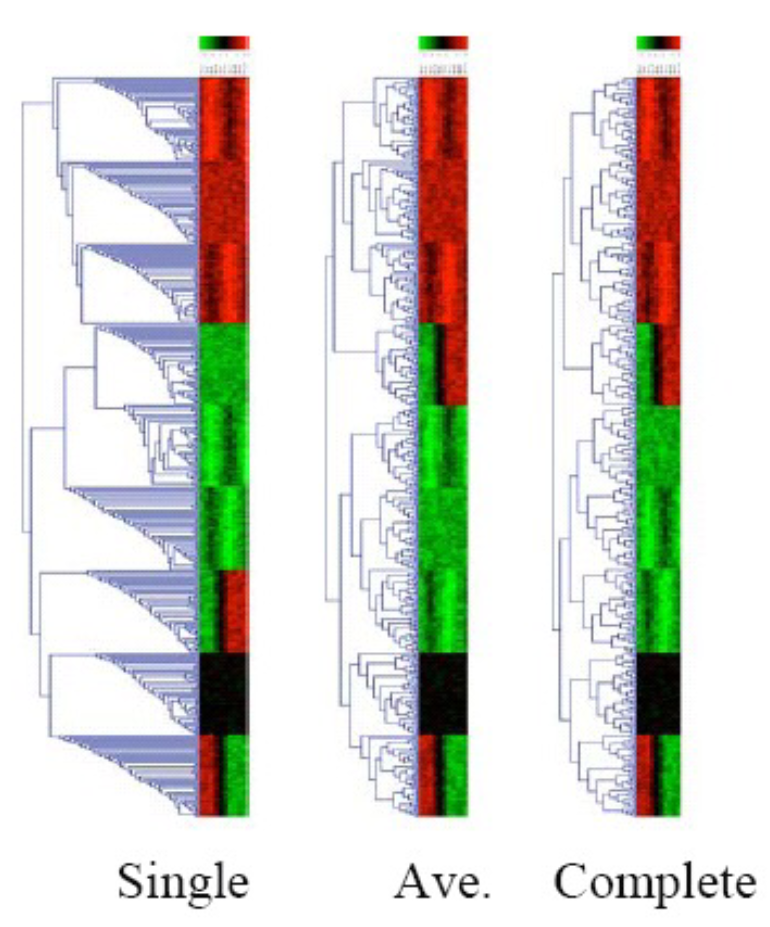
\includegraphics[width=0.8\textwidth]{img/8-linkage_effects.png}
    \end{minipage}
\end{figure}

\subsection{Cluster Quality: Modularity Q}
\label{subsec:modularity_q}

A critical challenge in hierarchical clustering is determining the optimal point to stop the agglomerative process. When should we stop linking nodes into broader communities? This requires a robust, objective measure of clustering goodness.

The standard metric for evaluating cluster quality is the \textbf{Modularity coefficient $Q$}. To compute $Q$, we treat the identified cluster assignments as categorical node labels and construct an $N \times N$ mixing matrix $E$ (where elements $e_{ij}$ represent the fraction of edges between community $i$ and community $j$).

Similar to the assortativity coefficient, Modularity measures the concentration of edges within modules compared to a random distribution. $Q$ is defined as the ratio of intra-community edges minus the expected inter-community edges:
$$Q = \sum_{i} \left( e_{ii} - \left( \sum_{j} e_{ij} \right)^2 \right) = \mathrm{Tr}(E) - \|E\|^2$$

\begin{figure}[H]
    \begin{minipage}{0.3\textwidth}
        \centering
        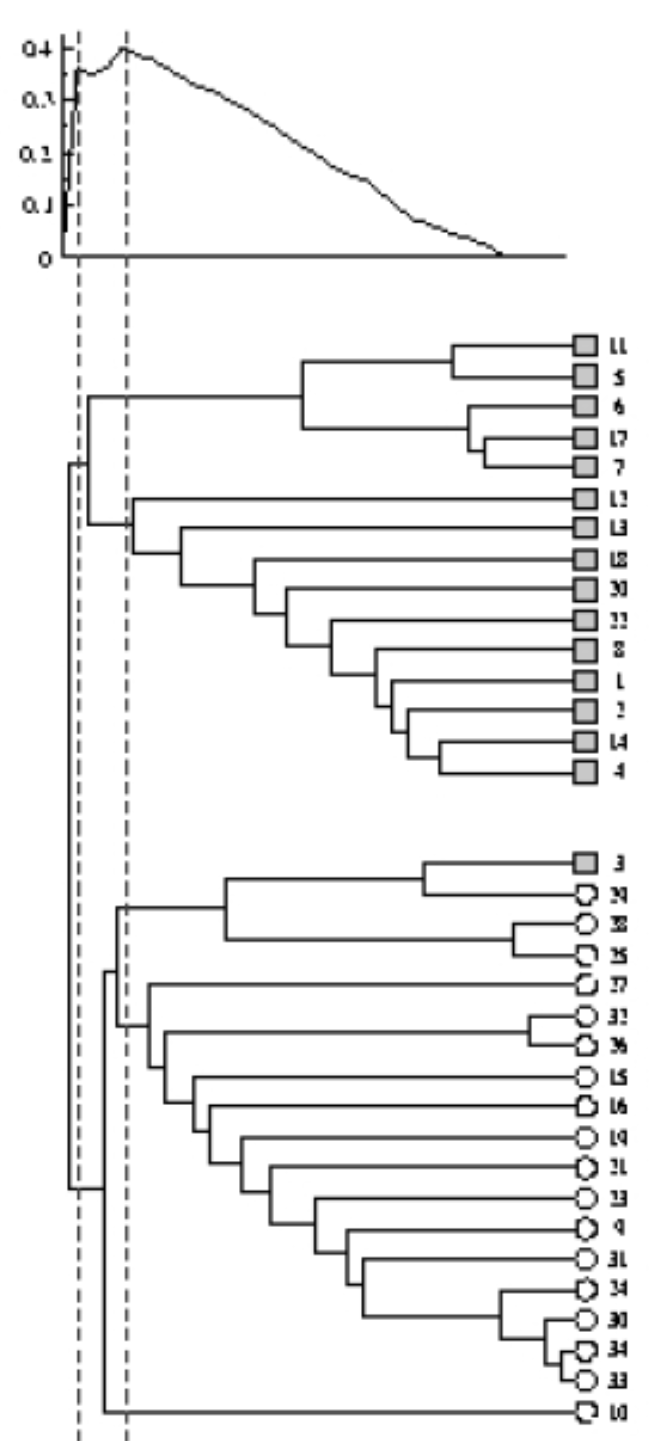
\includegraphics[width=0.8\textwidth]{img/8-dendrogram_cut.png}
    \end{minipage}
    \hfill
    \begin{minipage}{0.65\textwidth}
        The value of $Q$ indicates the strength of the community structure: a value approaching $1$ indicates an extremely strong community structure (good clustering), while a value near $0$ implies that the network's divisions are no better than random partitioning (bad clustering).

        Therefore, the optimal cut of a dendrogram corresponds to the hierarchical level that yields the maximal value of $Q$ (often a distinct local maximum in the modularity landscape).

        \caption{Dendrogram aligned horizontally with a corresponding line graph, depicting the goodness of split (Modularity Q) on the y-axis against the hierarchical split levels, clearly marking the optimal dendrogram CUT where Q reaches its maximum peak. }
    \end{minipage}
\end{figure}

\subsection{Clustering by Optimizing Modularity}
\label{subsec:clustering_optimizing_modularity}

Because Modularity provides a definitive mathematical criterion for community quality, community detection can be reframed as an optimization problem: finding the specific number and size of clusters that strictly maximize $Q$.

However, exploring all possible network partitions to find the absolute global maximum of $Q$ via brute force is an NP-complete problem, rendering it computationally intractable for large, complex networks.

Consequently, practical community detection algorithms frequently employ bottom-up heuristic approaches. These methods start with local communities or individual nodes as initial \textit{seeds} and recursively combine them, greedy-searching for merges that progressively yield the highest local increase in $Q$, stopping when no further combination improves the modularity score.

\subsection{Spectral Clustering Methods}
\label{subsec:spectral_methods}

In contrast to the agglomerative, bottom-up approach of hierarchical clustering, spectral clustering methods operate as top-down, divisive algorithms. These methods analyze the entire network macroscopically and progressively partition it into smaller, distinct clusters. The mathematical foundation of this approach lies in the spectral properties of the network's matrices, specifically the Laplacian matrix.

\subsubsection{The Laplacian Operator and Vibrational Modes}
\label{subsubsec:laplacian_vibrational}

The core mathematical object in spectral clustering is the Laplacian matrix, defined as $L = D - A$, where $D$ is the diagonal degree matrix and $A$ is the adjacency matrix.

The rationale behind using the Laplacian stems from its continuous analogue in physics: the Laplacian operator describes vibrational modes (eigenfunctions) across a domain, such as a continuous membrane. In the context of the Dirichlet problem, this is expressed as $\Delta \phi = \lambda \phi$ with boundary conditions $\phi|_{\partial} = f$.

When translated to the discrete topology of a network (provided there is an underlying metric structure), the eigenvectors of $L$ correspond to these discrete vibrational modes. The components of these eigenvectors have signs that indicate regions "vibrating" similarly. The nodal points—where the eigenvector components cross zero and change sign—act as natural separators or boundaries between different structural domains.

\begin{figure}[H]
    \centering
    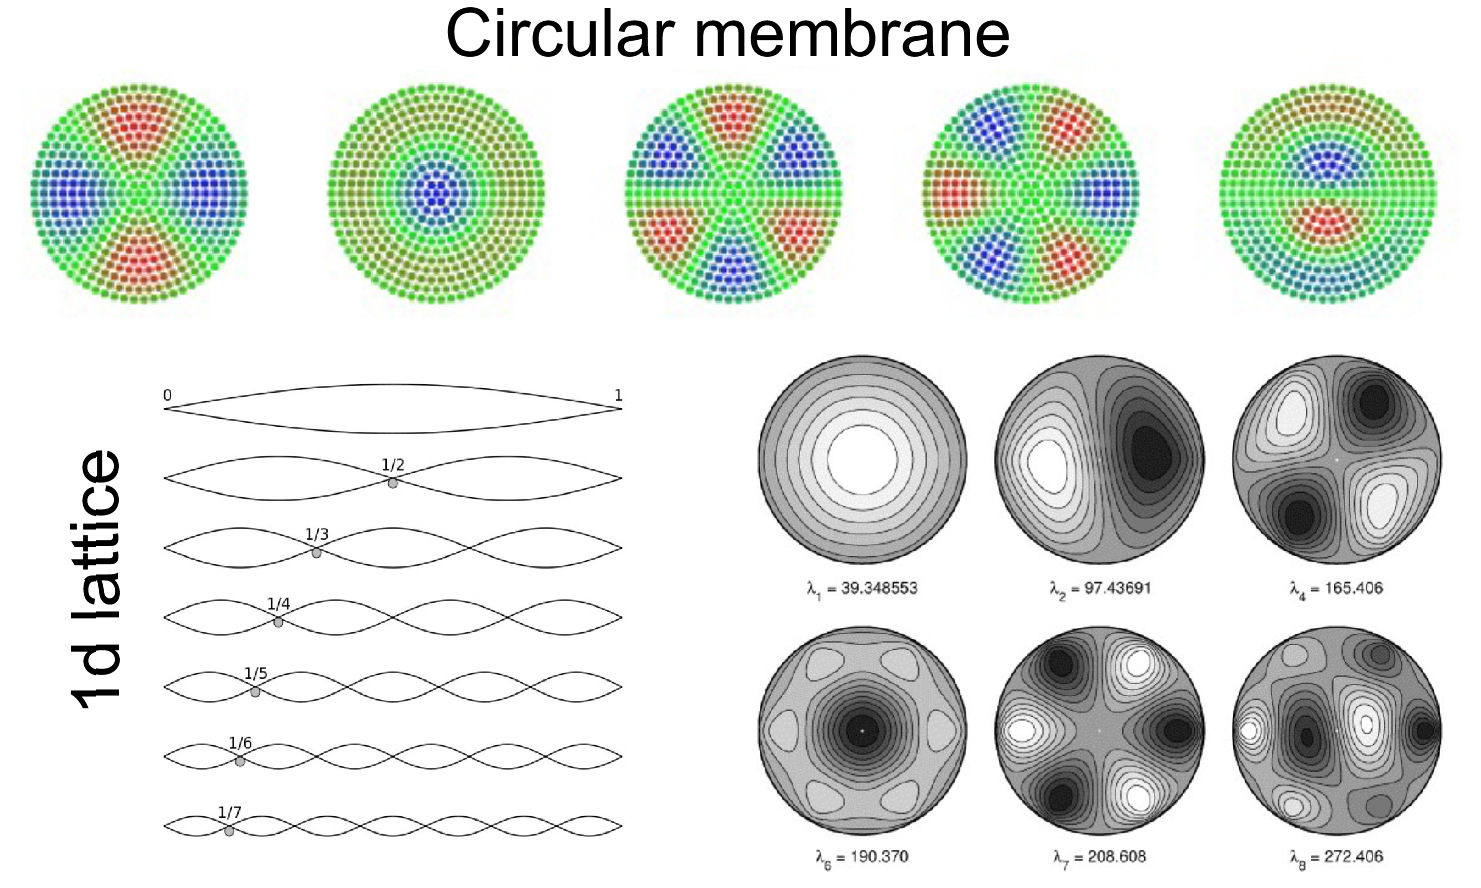
\includegraphics[width=0.8\textwidth]{img/8-laplacian_vibrations.png}
    \caption{Illustration of the Laplacian operator's role in spectral clustering. The top row depicts a circular membrane with varying vibrational modes, while the bottom row shows a 1D lattice with corresponding standing waves and their nodal points, alongside 2D circular nodal domain patterns corresponding to different eigenvalues.}
\end{figure}

\subsubsection{Laplacian Bisection and the Min-Cut Problem}
\label{subsubsec:min_cut_bisection}

The simplest application of spectral clustering is network bisection, which is intimately related to the Min-Cut problem. The objective of Min-Cut is to find a partition that divides the network into two subnetworks (communities $A$ and $B$) such that the number of links connecting the two partitions is minimized.

Ideally, we would assign discrete labels (e.g., $+1$ for community $A$ and $-1$ for community $B$) to every node to explicitly define the boundaries. However, finding the exact combinatorial minimum of boundary links is mathematically proven to be an NP-hard problem.

To bypass this computational intractability, spectral bisection provides a powerful approximate solution. The process involves minimizing the Rayleigh functional, which represents the cut size. If we consider a weighted network where $w_{ij}$ represents the link weight between nodes $i$ and $j$, the cut is defined as:

$$\mathrm{cut}(A, B) = \sum_{i \in A, j \in B} w_{ij} = \frac{1}{4} \sum_{i,j} w_{ij}(f_i - f_j)^2 = \frac{1}{2} f^T (D - W) f$$

Here, $f$ is the indicator vector containing the node assignments, and $W$ is the weight matrix (equivalent to $A$ in unweighted networks). To minimize this quadratic form, we utilize the Laplacian matrix $L$. The optimal approximate solution is derived by computing the eigenvector associated with the first non-zero eigenvalue of $L$, widely known as the \textbf{Fiedler vector}.

By looking simply at the \textit{sign} of the Fiedler vector's components, we can effectively bisect the network: nodes corresponding to positive components belong to community $A$, and those corresponding to negative components belong to community $B$. Because only the Fiedler vector needs to be computed, this method is computationally fast and can be recursively repeated on the resulting subgraphs to generate a cluster hierarchy.

\subsubsection{Optimal Subspace Selection}
\label{subsubsec:optimal_subspace}

While recursive bisection is efficient, standard spectral clustering can be generalized to identify multiple communities simultaneously. Instead of relying solely on the Fiedler vector, this approach selects a \textit{subspace} defined by the first $N$ Laplacian eigenvectors. Traditional clustering algorithms, such as K-means or standard hierarchical clustering, are then applied within this newly defined, low-dimensional spectral subspace.

The critical decision is determining the appropriate number of eigenvectors, $N$, to construct this optimal subspace. Selection criteria include:
\begin{itemize}
    \item \textbf{Physical Considerations}: Driven by the intrinsic dimensions of the studied problem (e.g., spatial constraints in proteins and DNA interactions).
    \item \textbf{Spectral Gap}: Analyzing the probability density function (pdf) of the eigenvalues to find a significant "gap," which naturally isolates the principal structural components of the network.
    \item \textbf{Geometric Constraints}: Mathematically, to represent separated clusters optimally without overlap, $N$ dimensions can separate at most $N+1$ clusters. This is analogous to forming an $N$-simplex (a generalization of a triangle into higher dimensions, or a convex hull).
\end{itemize}

Using too few dimensions leads to unresolved structures. For example, attempting to separate 4 distinct clusters using only 1 eigenvector will inevitably force at least two clusters to overlap on the 1D axis. However, projecting the same 4 clusters into a 2D subspace (using the first 2 eigenvectors) provides enough degrees of freedom to cleanly separate them.

\begin{figure}[H]
    \begin{minipage}{0.6\textwidth}
        \centering
        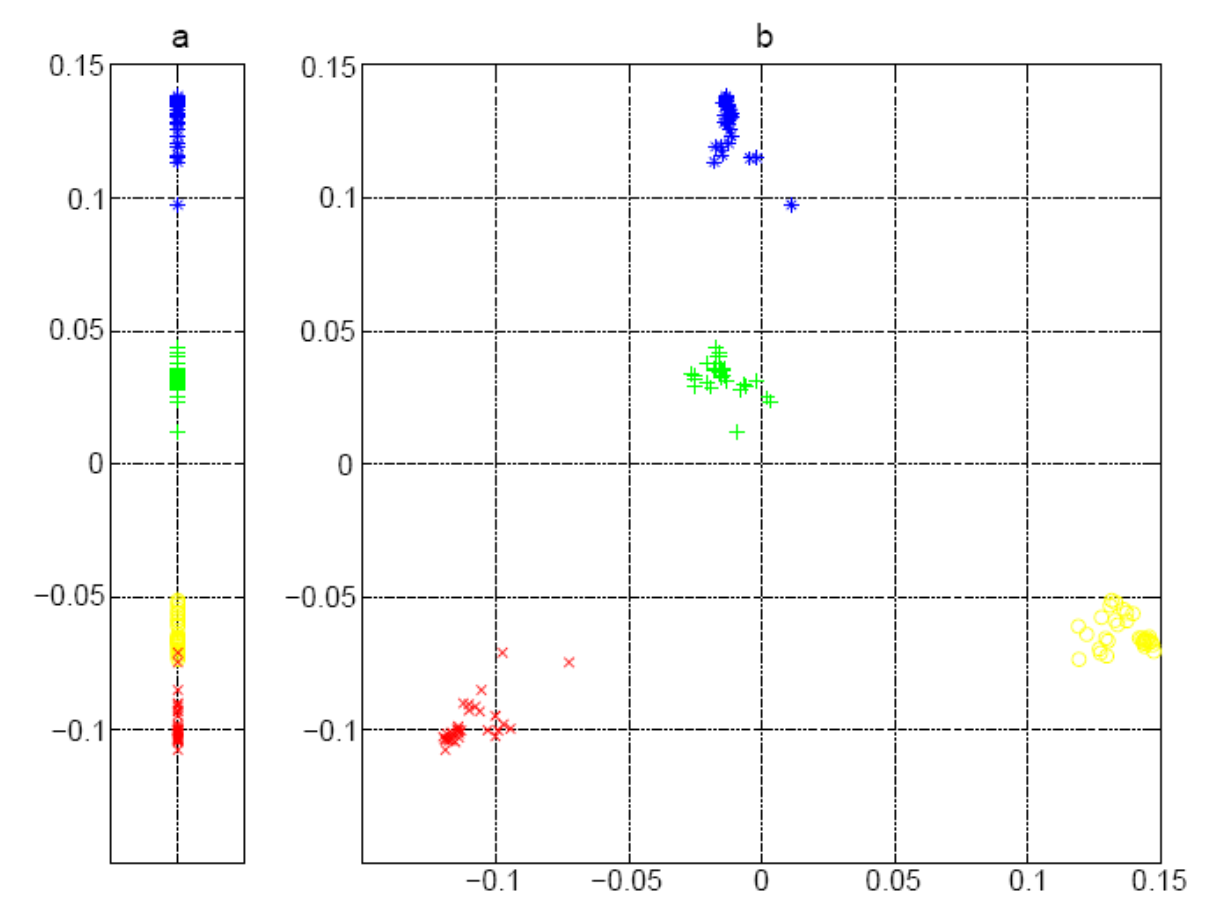
\includegraphics[width=0.8\textwidth]{img/8-eigenvector_projection.png}
    \end{minipage}
    \hfill
    \begin{minipage}{0.35\textwidth}
        \caption{Illustration of the impact of subspace dimensionality on cluster separation. The left panel shows 4 clusters projected onto a single eigenvector, resulting in significant overlap. The right panel demonstrates the same 4 clusters distinctly separated when projected onto a 2D space defined by the first two eigenvectors of the Laplacian.}
    \end{minipage}
\end{figure}

\subsubsection{Eigenvector Distributions and Network Bridges}
\label{subsubsec:eigenvector_bridges}

Spectral analysis also allows for the profound identification of network "bridges"—nodes that connect disparate communities and exhibit high betweenness centrality.

As the topological boundaries between communities begin to blur, the spectral signature of the network changes. Consider an empirical model with three communities where the intra-group connectivity density ($E_{ii}$) is fixed, but the inter-group connectivity ($E_{ij}$) progressively increases:
\begin{itemize}
    \item \textbf{Distinct Communities (Low $E_{ij}$)}: The eigenvector distribution shows tightly packed, distinctly separated point clouds corresponding to each community. Very few nodes act as bridges.
    \item \textbf{Emerging Overlap (Medium $E_{ij}$)}: As connections between groups increase, the network visually clumps closer together. In the spectral plot, the distinct point clouds begin to bleed into one another. The nodes located in the spaces between these clouds represent the inter-community bridges, which simultaneously exhibit highly elevated betweenness centrality scores.
    \item \textbf{Blended Network (High $E_{ij}$)}: When inter-group connectivity approaches the levels of intra-group connectivity, the distinct community structure completely collapses. The spectral distribution coalesces into a single centralized mass, indicating a lack of meaningful modularity, and the extreme betweenness centrality peaks disappear as paths diffuse uniformly across the homogeneous topology.
\end{itemize}

\begin{figure}[H]
    \centering
    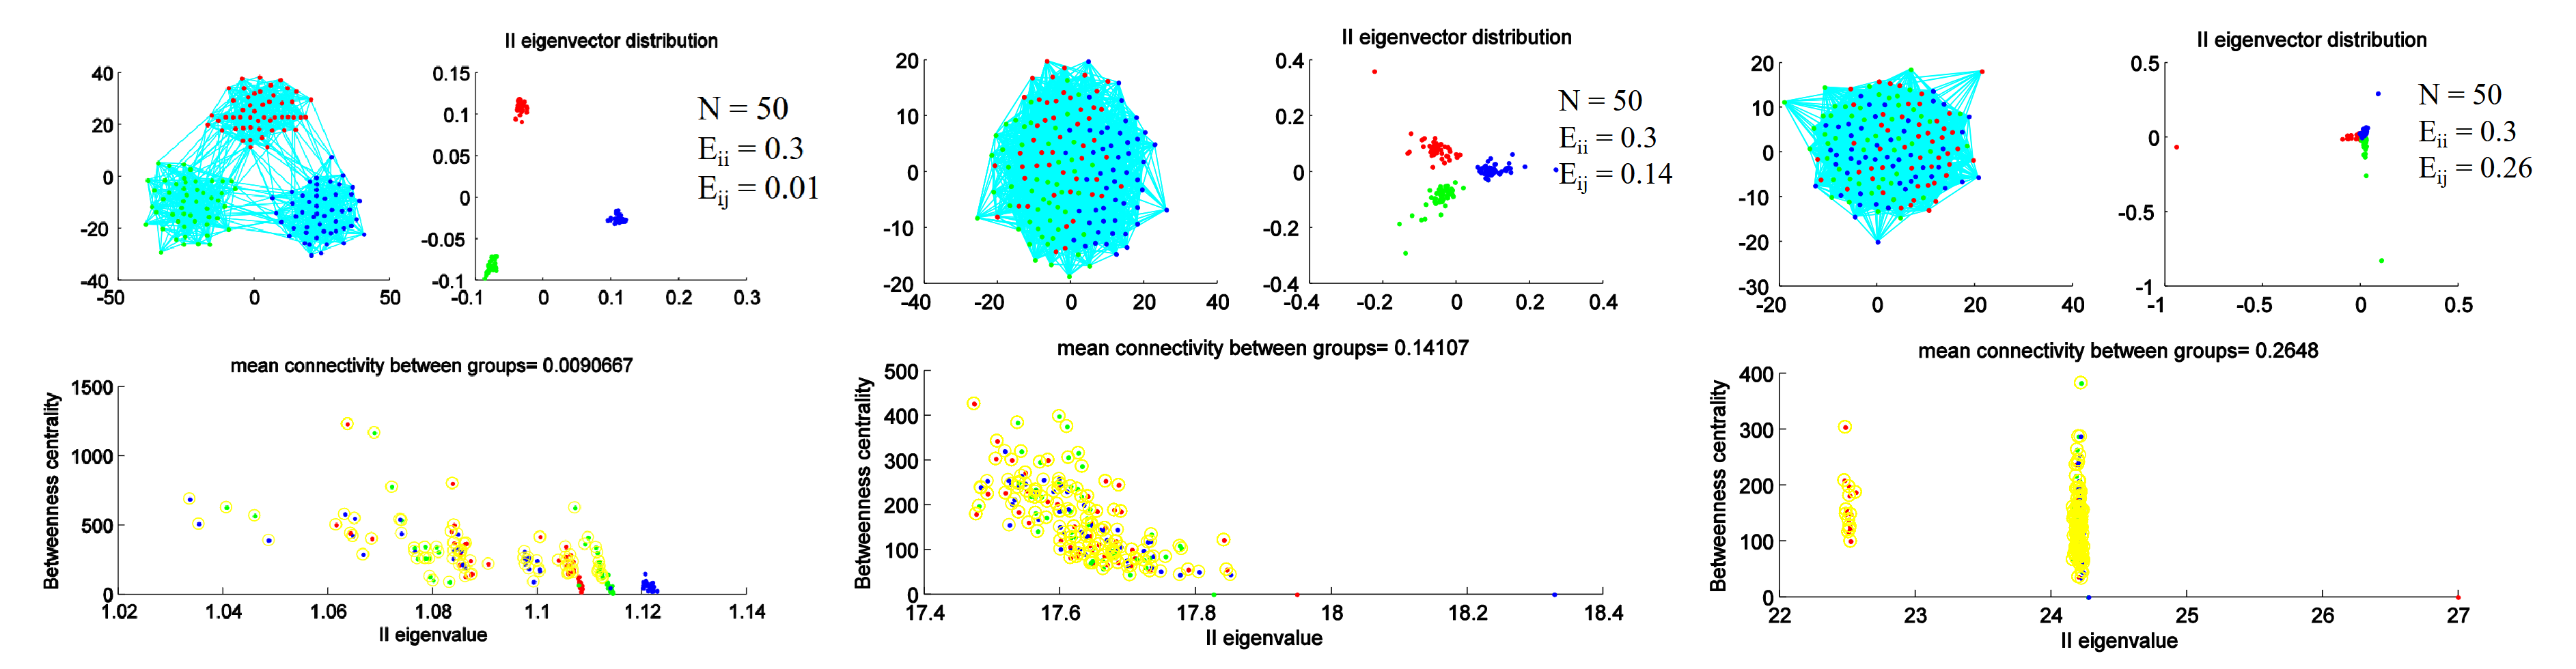
\includegraphics[width=\textwidth]{img/8-eigenvector_bridges.png}
    \caption{Three-panel image showing the "Eigenvector plot vs. BC-K bridges". Each panel contains three sub-plots: a network visualization (top left), the II eigenvector distribution (top right), and a scatter plot of Betweenness Centrality vs II eigenvalue (bottom). The sequence of panels from top to bottom show increasing inter-group connectivity ($E_{ij} = 0.01$, $0.14$, and $0.26$ respectively), visually demonstrating the degradation of community separation and the behavior of bridging nodes.}
\end{figure}

\subsection{Spectral Optimization of Modularity}
\label{subsec:spectral_optimization_modularity}

While spectral bisection using the standard Laplacian operator is highly effective for solving the Min-Cut problem, community detection is fundamentally about optimizing modularity, $Q$. We can reformulate the modularity optimization problem for network bisection using a spectral approach by introducing the Modularity Matrix, $B$.

\subsubsection{The Modularity Matrix and Bisection}

Consider the subdivision of a network into exactly two clusters. We can assign an index variable, or node label, $s_i \in \{+1, -1\}$ to each node $i$, representing its community membership. Under this bisection framework, the modularity $Q$ can be rewritten algebraically as:

$$Q = \sum_{i,j} \left( A_{ij} - \frac{k_i \cdot k_j}{\sum A_{ij}} \right) (1 + s_i \cdot s_j) = \vec{s}^T B \vec{s}$$

Here, we define the elements of the Modularity Matrix $B$ as:
$$B_{ij} = A_{ij} - \frac{k_i \cdot k_j}{2m}$$
where $2m = \sum_{i,j} A_{ij}$ represents the total weight (or twice the number of edges) in the network.

This formulation is highly intuitive:
\begin{itemize}
    \item The term $\frac{k_i \cdot k_j}{2m}$ represents the null model, specifically the expected random probability of a link existing between node $i$ (with degree $k_i$) and node $j$ (with degree $k_j$).
    \item The term $(1 + s_i \cdot s_j)$ acts as a filtering mechanism. It equals $2$ if nodes $i$ and $j$ belong to the same cluster (same sign), and it entirely cancels out (equals $0$) when nodes $i$ and $j$ belong to different clusters (opposite signs).
\end{itemize}

A critical mathematical property of the modularity matrix $B$ is that the sum of its elements evaluates strictly to zero. The constant term cancels out during summation:

$$\sum_{i,j} B_{ij} = \sum_{i,j} \left( A_{ij} - \frac{k_i \cdot k_j}{2m} \right) = 0$$

This simplification holds true because the sum of the adjacency matrix elements equals the total degree sum ($\sum_{i,j} A_{ij} = 2m$), and the sum of the degrees independent of each other also equals $2m$ ($\sum_i k_i = 2m$). Therefore, the expected edges precisely balance the actual edges over the entire network.

\subsubsection{The Generalized Laplacian and Eigenvalue Optimization}

The modularity matrix $B$ is a symmetric matrix featuring negative elements outside its main diagonal. Mathematically, it can be conceptualized as a "generalized weighted Laplacian". Unlike the standard Laplacian $L$, $B$ incorporates additional elements on the diagonal, acting as a "potential" $V$:

$$B \cdot \vec{x} = \mathcal{H} \cdot \vec{x} = L \cdot \vec{x} + V \cdot \vec{x}$$
where $V_{ij} = \delta_{ij} V_i$.

It is crucial to note that, unlike the standard Laplacian, the generalized Laplacian $B$ is \textit{not necessarily} semi-positive definite.

Because we have framed modularity as the quadratic form $Q = \vec{s}^T B \vec{s}$, finding the maximum modularity resolves into a Rayleigh eigenvalue problem. To maximize $Q$ under the discrete constraint that $s_i \in \{-1, +1\}$, we compute the leading eigenvector of $B$. We then choose the signs of the components of the vector $\vec{s}$ to perfectly align with the signs of the components in the eigenvector relative to the \textbf{maximum (most positive) eigenvalue}.

This presents a stark contrast to standard min-cut spectral partitioning:
\begin{itemize}
    \item \textbf{Min-Cut (Original Laplacian)}: Searches for eigenvectors related to the \textit{minimum} non-zero eigenvalue to minimize boundary links.
    \item \textbf{Modularity (Generalized Laplacian $B$)}: Searches for the eigenvector related to the \textit{maximum} eigenvalue to maximize internal community density relative to a random model.
\end{itemize}

Furthermore, the spectral properties of $B$ provide an organic stopping criterion for recursive algorithms: if the maximum eigenvalue of the modularity matrix for a given subgraph is strictly negative, it mathematically dictates that the sub-network is indivisible. Any further bisection would actively decrease the overall modularity $Q$.

\subsection{Clustering of Large Graphs: The Louvain Method}
\label{subsec:louvain_method}

While spectral methods provide elegant mathematical solutions, computing eigenvectors for massive networks is computationally prohibitive. For the clustering of exceedingly large graphs (e.g., networks exceeding $10^6$ nodes), highly efficient heuristic approaches are required. The most prominent among these is the \textbf{Louvain method}.

The Louvain algorithm is a greedy, agglomerative, bottom-up approach that recursively clusters nodes to construct a hierarchical dendrogram. It is exceptionally fast and is designed to find a local (or sub-optimal) maximum of modularity.

For an arbitrary number of communities, the global modularity $Q$ being optimized is formally expressed using the Kronecker delta function $\delta(c_i, c_j)$, which equals $1$ if the community of node $i$ ($c_i$) is the same as the community of node $j$ ($c_j$), and $0$ otherwise:

$$Q = \frac{1}{2m} \sum_{i,j} \left[ A_{ij} - \frac{k_i \cdot k_j}{2m} \right] \delta(c_i, c_j)$$

\subsubsection{Algorithm Mechanics}

The Louvain heuristic operates through a two-phase iterative process.

\textbf{Initialization Step:} The algorithm begins by assigning a distinct community to every single node in the network. In a network of $N$ nodes, there are initially $N$ communities.

\textbf{Iteration Cycle:}
\begin{enumerate}
    \item \textbf{Modularity Optimization (Local Moving):} The algorithm selects a node $i$ and evaluates the variation in modularity ($\Delta Q$) that would occur if node $i$ were removed from its current community and placed into the community of one of its immediate neighbors ($c_j$). The node is then moved to the neighboring community that yields the largest positive increase in $Q$. This process is applied sequentially to all nodes and is repeated repeatedly until no individual node movement can further increase the network's modularity. At this stage, a local maximum is reached.
    \item \textbf{Community Aggregation (Network Homomorphism):} Once local stability is achieved, the algorithm builds a new, macroscopic network. Each community identified in the first phase is collapsed into a single "super-node". Links between nodes within the same original community are summed to form a weighted self-loop on the super-node. Links between nodes in different communities are summed to form weighted edges between the corresponding super-nodes.
\end{enumerate}

These two steps—local optimization followed by network aggregation—constitute a single pass. The algorithm recursively repeats this entire cycle on the newly generated, smaller weighted networks until the global modularity $Q$ observes no further increases. The recursive nature naturally extracts the hierarchical structure of the complex system.